\documentclass[12pt,a4paper,openany,oneside]{book}

\usepackage{algpseudocode}
\usepackage{algorithm}
\usepackage{hyperref}
\usepackage{tikz}     
\usepackage{pgf-pie}  
\usepackage{subcaption}
\usepackage[italian]{babel}
\usepackage{placeins}
\usepackage[table]{xcolor}  
\usepackage{graphicx}       
\usepackage{array}          
\usepackage[utf8x]{inputenc}
\usepackage{graphicx}
\usepackage[font=small,labelfont=bf,tableposition=top]{caption}
\usepackage{listings}
\usepackage{courier}
\usepackage{amsmath}
\usepackage{framed}
\usepackage{xcolor}
\usepackage{multirow}
\usepackage[table]{xcolor}
\usepackage{amsmath}
\usepackage{amssymb}

\lstset{
         language=C++,
         basicstyle=\footnotesize\ttfamily,
         numbers=left,           
         numberstyle=\tiny,       
         numbersep=5pt,        
         tabsize=5,                 
         extendedchars=true,         
         breaklines=true,
         keywordstyle=\textbf,           
         stringstyle=\color{white}\ttfamily,
         showspaces=false,       
         showtabs=false,           
         xleftmargin=17pt,
         framexleftmargin=17pt,
         framexrightmargin=5pt,
         framexbottommargin=4pt,
         showstringspaces=false          
}
 
\addto\captionsitalian{\renewcommand{\lstlistingname}{Codice}}

\setcounter{tocdepth}{3} % fa apparire le subsubsection nell'indice
\setcounter{secnumdepth}{3} % e le numera

\definecolor{sqcolor}{HTML}{789ECC}
\definecolor{cocolor}{HTML}{C23A21}
\definecolor{tgcolor}{HTML}{02BF3D}

\begin{document}

%Inserisce qui il frontespizio
\input{parts/frontespizio} %<- richiama il file "parts/titlepage.tex" che contiene il frontespizio

\bibliographystyle{unsrt}
\title{Titolo Della Tesi}
\author{Nome Autore}

%Inserisce qui l'abstract
\chapter*{Abstract} % l'asterisco dopo chapter serve per visualizzare il titolo senza numerazione

In questa tesi si analizza l'uso dei video egocentrici per lo studio del comportamento umano in scenari operativi, con particolare attenzione alla gestione delle interazioni tra mani e oggetti. Viene presentato AMEGO \cite{goletto2024amego}, un framework semantic-free per la strutturazione di una memoria capace di fornire informazioni basate su dati visuali-temporali.

Il lavoro prevede la realizzazione di un benchmark in un contesto industriale, utilizzando il dataset \textit{ENIGMA-51} \cite{ragusa2023enigma51}, opportunamente adattato per valutare le prestazioni del modello in un dominio differente rispetto a quello originariamente considerato \cite{Damen2021PAMI}. Le valutazioni mostrano limiti nella distinzione tra oggetti visivamente simili, sottolineando la necessità di strategie più robuste per il \textit{clustering} e l'organizzazione degli oggetti.

Nonostante queste limitazioni, AMEGO rappresenta una base solida per l'analisi dei video egocentrici, consentendo di studiare diversi aspetti che coinvolgono l'operatore umano e offrendo spunti per sviluppi futuri volti a migliorare la robustezza e la generalizzazione del modello, anche in contesti e dataset differenti.

%Genera l'indice
\tableofcontents

\chapter{Introduzione}

Negli ultimi anni i dispositivi indossabili per la registrazione di video in prima persona hanno conosciuto una diffusione sempre più ampia. Strumenti come \emph{smart glasses}, \emph{body cameras}, \emph{action cameras} hanno reso possibile la cattura di flussi visivi continui dal punto di vista diretto dell'utilizzatore, dando origine a quella che viene comunemente definita come \emph{egocentric video}. Questa modalità di acquisizione ha suscitato un forte interesse \cite{NUNEZMARCOS2022175} non solo per le applicazioni pratiche, che spaziano dallintrattenimento personale alla sicurezza e al monitoraggio di attività lavorative, ma anche per le sfide che pone in termini di analisi e interpretazione dei contenuti.

\begin{figure}[ht]
    \centering
    \begin{minipage}{0.3\linewidth}
        \centering
        \includegraphics[width=\linewidth]{Images/meta_glass.png}\\
        (a) Smart glasses
    \end{minipage}
    \hfill
    \begin{minipage}{0.3\linewidth}
        \centering
        \includegraphics[width=\linewidth]{Images/gopro.png}\\
        (b) Action camera
    \end{minipage}
    \hfill
    \begin{minipage}{0.3\linewidth}
        \centering
        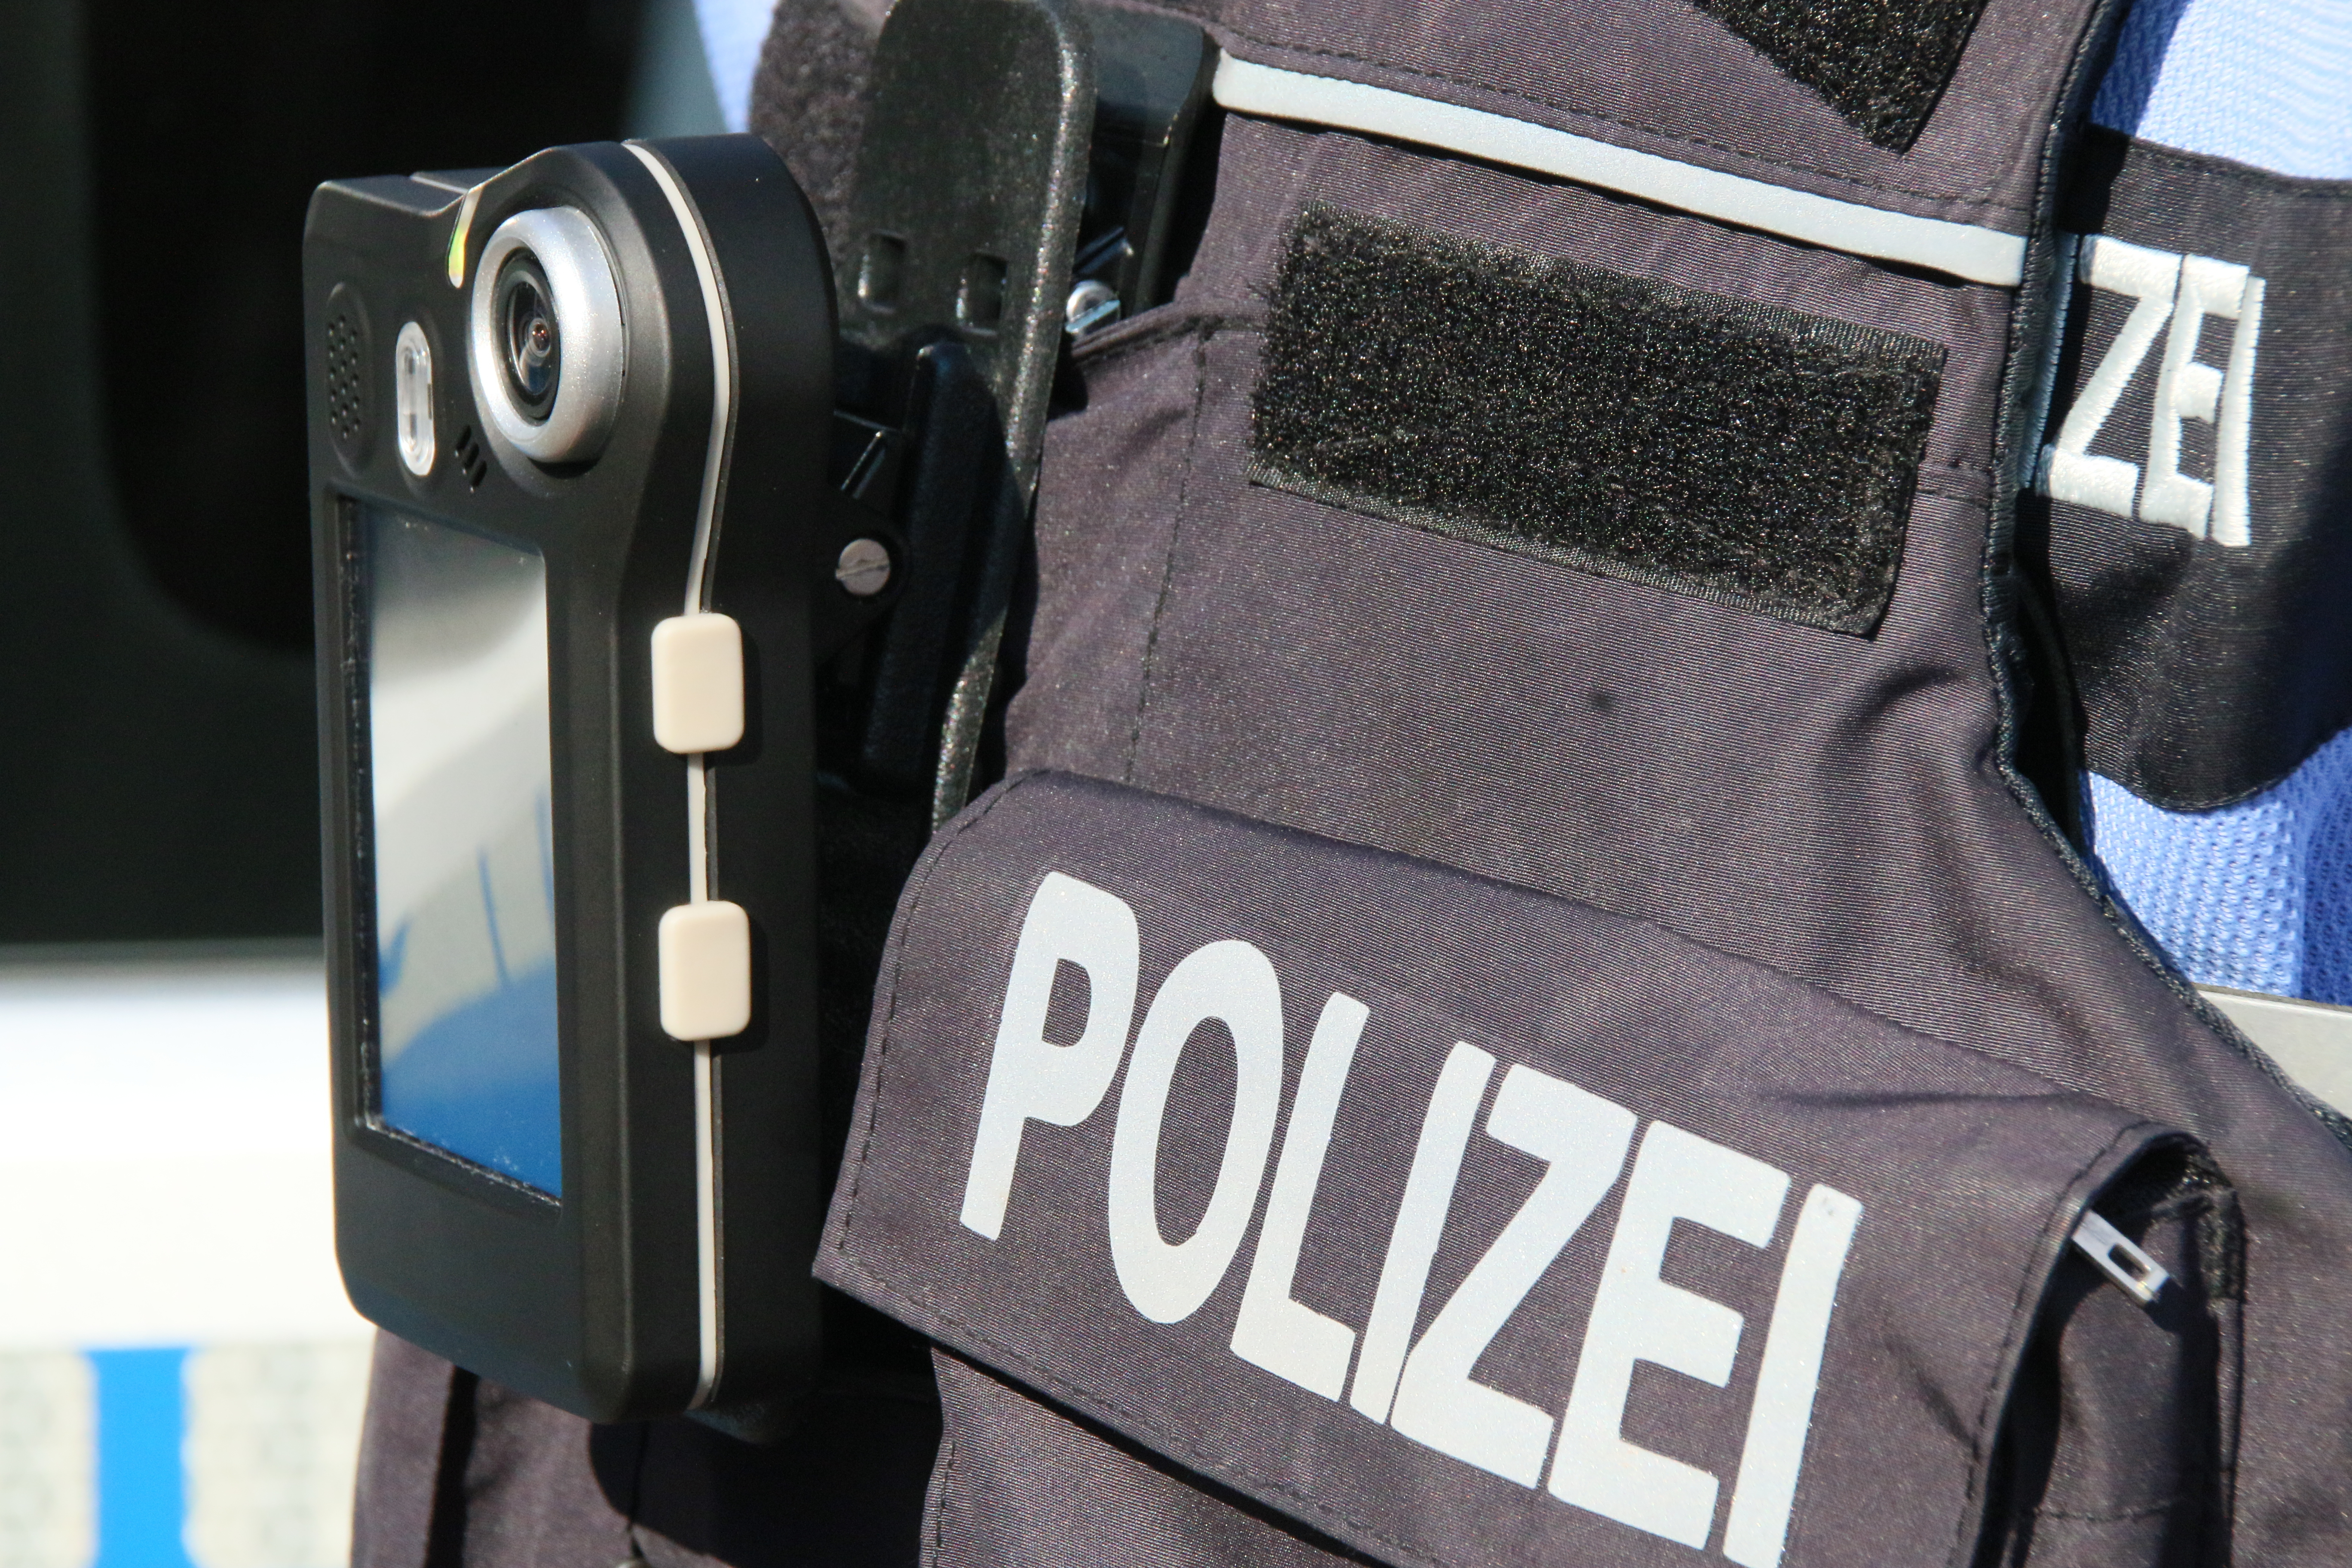
\includegraphics[width=\linewidth]{Images/bodycamera.png}\\
        (c) Body camera
    \end{minipage}
    \caption{Esempi di dispositivi indossabili per la cattura di video egocentrici}
    \label{fig:dispositivi_egocentrici}
\end{figure}

L'adozione di tali dispositivi è stata favorita dalla loro versatilità: da un lato vengono utilizzati per scopi ricreativi e per la condivisione di esperienze personali, dall'altro trovano applicazione in contesti professionali e industriali, dove consentono di documentare procedure complesse e migliorare i processi di formazione e supervisione. Ciò che rende peculiari i video egocentrici è la loro capacità di catturare dettagli e prospettive uniche, fornendo una visione diretta dell'attività di chi li indossa.

Il principale ostacolo all'analisi di questi contenuti risiede nella loro natura non strutturata. I video in prima persona possono essere considerati come veri e propri flussi di coscienza visivi: lunghi, frammentati, privi di un'organizzazione narrativa chiara e difficili da interpretare. La presenza di movimenti rapidi della fotocamera, variazioni di illuminazione e interazioni simultanee con più oggetti rende complicata l'estrazione di significato. Un'annotazione manuale completa non è praticabile, sia per la mole di dati prodotta sia per la complessità dei contenuti.

Da questa problematica emerge la necessità di costruire una “memoria artificiale” capace di trasformare i video egocentrici in rappresentazioni strutturate e interrogabili. Questa tesi prende avvio dall'analisi dei principali contributi degli elementi che vanno a formare un eventuale memoria artificiale, per poi focalizzarsi su AMEGO \cite{goletto2024amego}, acronimo di \emph{Active Memory of the EGOcentric video}, un sistema sviluppato per organizzare e rendere interrogabili i contenuti visivi in prima persona e attualmente considerato stato dell'arte nel suo ambito \cite{goletto2024amego}.

Il contributo di questo lavoro consiste nella valutazione di AMEGO in un contesto diverso rispetto a quello in cui è stato originariamente validato. Inizialmente il sistema è stato sperimentato sul dataset \emph{ EPIC KITCHENS }\cite{Damen2021PAMI}, una collezione di video ambientati in cucine domestiche. In questa tesi, invece, viene preso in esame il dataset \emph{ENIGMA-51} \cite{ragusa2023enigma51}, un dataset egocentrico acquisito in scenari industriali, in cui diversi operatori hanno seguito procedure guidate per eseguire attività di riparazione di quadri elettrici. La differenza tra i due domini rende lo studio particolarmente interessante, in quanto consente di valutare la capacità di AMEGO di generalizzare a contesti applicativi mai visti.

In ambito industriale, l'analisi dei video egocentrici e la gestione della concurrency assumono un ruolo fondamentale per ottimizzare diversi aspetti operativi. In particolare, si possono individuare due benefici principali:
\begin{itemize}
    \item \textbf{Affidabilità del processo:} garantire che le operazioni vengano eseguite nell'ordine corretto consente di ottimizzare i flussi produttivi e di ridurre il rischio di errori umani, assicurando maggiore coerenza nelle procedure.
    \item \textbf{Sicurezza dei lavoratori:} monitorare in tempo reale l'uso corretto dei dispositivi di protezione individuale (DPI) oppure verificare la collocazione di componenti critici. Ad esempio, un materiale pericoloso come un condensatore ad alta tensione deve essere riposto in aree designate per prevenire incidenti.
\end{itemize}

Un aspetto centrale analizzato in questo lavoro riguarda la gestione della \emph{concurrency}, intesa come la capacità di riconoscere non solo con quali altri oggetti un determinato strumento viene utilizzato in simultanea, ma anche in quali contesti o aree operative tale oggetto viene impiegato.
Nei capitoli successivi verranno prima esaminati gli strumenti e le metodologie attualmente presenti in letteratura, che costituiscono le basi per lo sviluppo di sistemi di memoria artificiale per video egocentrici. Successivamente saranno illustrate nel dettaglio le caratteristiche di AMEGO \cite{goletto2024amego} e le sperimentazioni condotte sul dataset ENIGMA-51 \cite{ragusa2023enigma51}, con l'obiettivo di valutare fino a che punto il sistema possa essere adattato a contesti applicativi diversi da quelli per cui è stato originariamente progettato.
\chapter{Lavori correlati}
\section{Long video understanding}
La comprensione di video di lunga durata riguarda l'analisi e l'interpretazione di contenuti visivi che possono estendersi per diversi minuti o addirittura ore. Questi video richiedono metodi capaci di catturare sequenze temporali complesse e le interazioni tra più oggetti e persone, il che rende la gestione di flussi video così lunghi particolarmente impegnativa dal punto di vista computazionale.

Per affrontare la sfida della comprensione di video di lunga durata, sono stati sviluppati benchmark specifici che mettono alla prova la capacità dei modelli di gestire sequenze temporali estese e interazioni complesse. Tra i più rilevanti troviamo EgoSchema \cite{mangalam2023egoschemadiagnosticbenchmarklongform}, un dataset egocentrico con video della durata massima di circa tre minuti, progettato per diagnosticare azioni quotidiane articolate in più passaggi. I video includono azioni come preparare un oggetto, combinarlo con altri strumenti o spostarlo tra diverse aree operative, spesso con oggetti in movimento e interazioni parzialmente sovrapposte. I modelli devono quindi seguire la coerenza temporale, riconoscere pattern ricorrenti, e inferire correttamente le relazioni tra oggetti e azioni, mantenendo una rappresentazione accurata di sequenze multi-step.

ReST \cite{Yang_2023_CVPR} propone invece scenari industriali e scientifici più complessi, con video più lunghi in cui interagiscono simultaneamente più strumenti, oggetti e operatori. I compiti richiesti includono il tracciamento di oggetti su intervalli temporali estesi, il riconoscimento di interazioni multiple e la comprensione delle relazioni spaziali tra componenti e strumenti. 

Diversi approcci sono stati sviluppati per la comprensione di video di lunga durata. Alcuni trattano il problema come un task di \emph{natural language question answering}, generando prima dei sottotitoli o descrizioni automatiche del video e utilizzando LLM per rispondere a domande specifiche \cite{ma2024drvideodocumentretrievalbased, park2025framesusefulefficientstrategies, wang2024videoagentlongformvideounderstanding, wang2024lifelongmemoryleveragingllmsanswering, wang2025videotreeadaptivetreebasedvideo, wu2022memvitmemoryaugmentedmultiscalevision}. Altri approcci integrano direttamente LLM con un encoder video, sfruttando le capacità di comprensione e generazione dei modelli linguistici per elaborare sequenze visive estese in maniera coerente \cite{li2024llmsmeetlongvideo, qian2024streaminglongvideounderstanding, ren2024timechattimesensitivemultimodallarge, song2024moviechatdensetokensparse}.

\section{Structured video representations}

Con \emph{rappresentazione strutturata} si intende l'insieme di tecniche volte a organizzare un video non come una semplice sequenza di frame, ma come una struttura semantica in grado di esplicitare le relazioni tra gli elementi presenti nella scena. Questo approccio consente di passare da una descrizione puramente visiva a una rappresentazione schematica e strutturata, che rende possibile interrogare i video in maniera più efficace, permettendo di estrarre informazioni mirate.

Un filone centrale della ricerca si è concentrato sullo studio delle relazioni contestuali, investigando in particolare i legami tra oggetti e attori \cite{arnab2021unifiedgraphstructuredmodels, baradel2018objectlevelvisualreasoning, cong2021spatialtemporaltransformerdynamicscene, jain2016structuralrnndeeplearningspatiotemporal, ji2019actiongenomeactionscomposition, ma2018attendinteracthigherorderobject, sun2018actorcentricrelationnetwork, wang2018videosspacetimeregiongraphs}. Parallelamente, sono stati proposti modelli basati su grafi per rappresentare le dipendenze tra azioni, al fine di catturare la dimensione temporale e causale dei comportamenti.

Alcuni lavori hanno cercato di spingersi oltre, introducendo strategie più specifiche. Un esempio è UnweaveNet \cite{price2022unweavenetunweavingactivitystories}, che raggruppa i video in \emph{activity threads}, ossia insiemi di clip collegati logicamente che consentono di separare e ricostruire le diverse “storie” di attività intrecciate all'interno di una sequenza più lunga. Un altro contributo rilevante è l'introduzione dei cosiddetti \emph{egocentric scene graphs} \cite{rodin2023actionscenegraphslongform}, strutture orientate a rappresentare in modo esplicito le interazioni tra il soggetto che indossa la videocamera e gli oggetti presenti nell'ambiente.

Nonostante questi progressi, tali approcci risultano ancora limitati, poiché tendono a catturare soltanto alcuni aspetti delle attività. In particolare, faticano a integrare in un unico modello le molteplici dimensioni tipiche dei video egocentrici: le interazioni con gli oggetti, i luoghi chiave in cui esse avvengono e le interdipendenze tra questi elementi. Questa mancanza di completezza riduce la capacità di ottenere rappresentazioni realmente efficaci per la comprensione e la memorizzazione dei flussi visivi in prima persona.

\section{Video summarization}

Il riassunto del video ha come obiettivo la generazione di una versione ridotta di un video, tipicamente attraverso l'estrazione di \emph{key frames} o \emph{key shots} che ne catturino i momenti salienti. Gli approcci proposti in letteratura variano in funzione degli elementi ritenuti rilevanti per la sintesi: alcuni si focalizzano sulla presenza e sul ruolo delle persone o degli oggetti all'interno della scena \cite{inproceedings0}, altri privilegiano la rilevazione di eventi significativi \cite{Lu_2013_CVPR}, mentre ulteriori metodi considerano anche caratteristiche estetiche dei fotogrammi chiave per selezionare i contenuti più rappresentativi \cite{inproceedings1}. 

Accanto a questi, sono stati introdotti approcci in grado di generare i riassunti in modalità \emph{online}, ossia durante la riproduzione del flusso video, consentendo una sintesi in tempo reale \cite{Lin_2015_ICCV_Workshops,Zhao_2014_CVPR}. Tuttavia, tali tecniche non costruiscono una rappresentazione strutturata del video e risultano spesso sensibili al rumore prodotto dai modelli di rilevamento, mancando di un'efficace integrazione della dimensione temporale.

Un contributo particolarmente rilevante in questa direzione è rappresentato da \cite{Xiong_2015_ICCV}, che introduce una modalità di sintesi per i video egocentrici basata su attori, eventi, luoghi e oggetti. Questo approccio permette di interrogare i contenuti lungo diverse dimensioni, anche combinandole attraverso operatori booleani. Ciononostante, il metodo rimane in gran parte vincolato al riconoscimento di attrazioni predefinite e di oggetti visivamente distinti, risultando meno efficace in scenari affollati e caotici.
\chapter{Metodo - AMEGO} 
AMEGO, acronimo di \emph{Active Memory of the EGOcentric video}, è concepito per trasformare un video egocentrico lungo e non strutturato in una memoria capace di descrivere in modo completo le interazioni del soggetto con oggetti e luoghi, e al tempo stesso interrogabile per recuperare i segmenti temporali in cui un oggetto è stato utilizzato, una location visitata o entrambe le condizioni si sono verificate congiuntamente.

Un aspetto cruciale che distingue AMEGO da altri approcci riguarda la sua natura \emph{semantic-free}.  
Gli oggetti e le location non vengono legati ad una tassonomia fissa di etichette o ad un vocabolario prestabilito. Essi vengono invece rappresentati direttamente sulla base delle caratteristiche visive, consentendo così una distinzione più fine e dettagliata tra le diverse istanze. Questo approccio permette al sistema di adattarsi a contesti nuovi senza la necessità di ridefinire un insieme di categorie predefinite.

\section{Decomposizione del video}
Dato un video egocentrico $\mathcal{V}$, esso viene scomposto in due elementi fondamentali:

\begin{itemize}
    \item \textbf{Hand-Object Interaction (HOI) tracklets}, indicati con $\Theta$: ciascun HOI tracklet\footnote{\textbf{Tracklet}: sequenza di bounding box che identifica in modo coerente la traiettoria o l’interazione di un oggetto nel tempo.} descrive in maniera spazio-temporale un oggetto che interagisce in modo consistente con almeno una mano del soggetto. Ogni tracklet è caratterizzato da bounding boxes\footnote{\textbf{Bounding box}: regione rettangolare che delimita un oggetto in un singolo frame del video.} spazio-temporali e dalle corrispondenti feature visive\footnote{\textbf{Feature visive}: rappresentazioni numeriche delle proprietà visive di un oggetto}.
    
    \item \textbf{Location segments}, indicati con $\mathcal{L}$: ogni elemento corrisponde a un intervallo temporale in cui il soggetto si trova in un determinato luogo e vi svolge interazioni. L’interesse è focalizzato sulle cosiddette \emph{activity-centric-zones}, ossia i luoghi in cui avvengono le principali interazioni con gli oggetti.
\end{itemize}

Combinando gli \emph{HOI tracklets} con i \emph{Location segments} si ottiene una memoria strutturata in grado di eseguire i compiti discussi in precedenza.

\section{Costruzione della memoria}
La memoria viene definita come:
\[
\mathcal{E} = \{\mathcal{O}, \mathcal{L}\}
\]
dove:
\begin{itemize}
    \item $\mathcal{E}$: AMEGO
    \item $\mathcal{O}$: insieme di HOI tracklets
    \item $\mathcal{L}$: insieme dei Location Segments.
\end{itemize}

Questa memoria viene costruita \emph{online}, eliminando la necessità di ri-processare continuamente informazioni passate.

\subsection{Object interaction tracklets}
Gli \emph{HOI tracklets}, indicati con $\mathcal{O}$ rappresentano sequenze di interazioni tra le mani del soggetto e gli oggetti presenti nel video. Formalmente, possiamo definire l'insieme degli HOI tracklets come:

\[
\mathcal{O} = \{ o_1, o_2, \dots, o_n \}
\]

dove ciascun tracklet $o_i \in \mathcal{O}$ è una tupla:

\[
o_i = (t_s, t_e, b_t, h, \text{id})
\]

con:
\begin{itemize}
    \item $t_s$: istante di inizio dell'interazione
    \item $t_e$: istante di fine dell'interazione
    \item $b_t$: sequenza di bounding box che raffigurano l'oggetto
    \item $h$: lato della mano che compie l'interazione (sinistra o destra)
    \item $\text{id}$: identificatore dell'istanza dell'oggetto associato al tracklet
\end{itemize}

La costruzione della memoria $\mathcal{O}$ avviene in maniera iterativa, processando il video frame per frame tramite una pipeline composta da tre fasi principali:

\begin{enumerate}
    \item \textbf{Initialisation:} individuazione dei possibili nuovi HOI tracklets.
    \item \textbf{Updating:} aggiornamento dei tracklets attivi\footnote{\textbf{Tracklet attivi}: tracklets che stanno effettivamente registrando un’interazione in corso tra la mano del soggetto e l’oggetto}, corrispondenti alle interazioni in corso.
    \item \textbf{Assignment and storing:} i tracklets terminati \footnote{\textbf{Tracklet terminato}: l’azione per cui veniva considerato attivo è terminata} vengono archiviati nella memoria $\mathcal{E}$ e viene assegnata loro l’istanza oggetto corrispondente.
\end{enumerate}


\subsection*{Inizializzazione}
La prima fase consiste nell’individuazione dei nuovi \emph{HOI tracklets}. Per questo utilizziamo un detector di \emph{hand-object-interaction} \emph{class-agnostic}\footnote{\textbf{class-agnostic detector}: non fa distinzione tra classi predefinite di oggetti, ma identifica interazioni tra mani e oggetti basandosi su caratteristiche visive generiche} \cite{shan2020understandinghumanhandscontact}, che fornisce insiemi di bounding box attive per oggetti e mani, denotati rispettivamente come $\mathcal{B}_t^o$ e $\mathcal{B}_t^h$.

Un nuovo \emph{HOI tracklet} $o_i$ viene inizializzato per ciascuna nuova hand-object-interaction rilevata. Ogni tracklet è definito come una sequenza di almeno $s_o$ bounding box che mostrano un forte sovrapposizione spaziale all’interno di una finestra temporale di $w_s$ frame.

\begin{figure}[ht]
    \centering
    \includegraphics[width=0.6\textwidth]{Images/init.png}
    \caption{Fase di inizializzazione}
    \label{fig:init}
\end{figure}

Questo filtraggio spazio-temporale permette di ridurre il rumore derivante dall’applicazione indipendente del rilevatore su ciascun frame. Considerando la durata naturale delle interazioni mano-oggetto, è possibile identificare in modo affidabile i nuovi tracklets attivi, garantendo coerenza spaziale e temporale nelle rilevazioni.  

Il tracklet $o_i$ viene ora considerato \emph{attivo} e aggiunto alla memoria $\mathcal{O}$.  

Per ciascun frame successivo, calcoliamo l’\emph{Intersection over Union (IoU)}\footnote{\textbf{Intersection over Union (IoU)}: misura di sovrapposizione tra due bounding box, calcolata come il rapporto tra l'area di intersezione e l'area di unione dei due rettangoli.} tra i bounding box degli oggetti che interagiscono con la stessa mano. I bounding box che superano una soglia $\theta$ vengono assegnati al tracklet $o_i$. Se non è possibile assegnare nuovi bounding box al tracklet, questo viene considerato \emph{terminato}.

\subsection*{Updating}

Questa fase mira a catturare l’intera durata dell’interazione e contemporaneamente a seguire tutte le occorrenze spaziali dell’oggetto.

Sebbene i rilevatori di HOI a livello di singolo frame siano sufficienti per identificare nuove interazioni, essi non sono in grado di estendere in modo affidabile i tracklets quando mani o oggetti escono dal campo visivo egocentrico. Per questo motivo, viene utilizzato un off-the-shelf \emph{single-object tracker (SOT)}\footnote{\textbf{Single-Object Tracker (SOT)}: permette di seguire un singolo oggetto nel tempo, stimandone la posizione frame per frame anche in assenza di rilevazioni dirette.} \cite{tang2023egotrackslongtermegocentricvisual}.  

\begin{figure}[ht]
    \centering
    \includegraphics[width=0.6\textwidth]{Images/update.png}
    \caption{Fase di updating}
    \label{fig:update}
\end{figure}

Per ogni tracklet attivo $o_i$ viene inizializzato un SOT. Consideriamo il tracklet $o_i$ terminato se non sono presenti rilevazioni associate $\mathcal{B}^o$ per $e_o$ frame consecutivi, mentre la mano $h$ rimane visibile, in quanto quando la mano esce dal campo visivo è probabile che stia ancora tenendo l’oggetto.

L’output del SOT produce un track $\tau_{o_i}$ spazio-temporale che segue la posizione dell’oggetto, ma non contiene informazioni sull’interazione stessa. A questo punto, $o_i$ combina le informazioni relative alla durata temporale (start e end time) e ai bounding box spaziali dell’oggetto attivo, sfruttando sia la rilevazione HOI a livello di frame sia il tracciamento SOT.

\subsection*{Assignment and storing}

Come definito in precedenza, ogni HOI tracklet $o_i$ deve essere associato a una specifica istanza di oggetto. Per farlo, confrontiamo $o_i$ con le istanze già presenti nella memoria.  

In particolare, data l'insieme di HOI tracklets già memorizzati al tempo $t$, denotato $\mathcal{O}_t$, e l'insieme dei tracciamenti SOT osservati nello stesso istante, $\tau_t$, verifichiamo se $o_i$ possa essere associato a un'istanza esistente o se sia necessario crearne una nuova. Per effettuare il confronto, calcoliamo prima le feature visive di $o_i$:

\[
f(o_i) = \frac{1}{|\mathcal{V}_{o_i}|} \sum_{k \in \mathcal{V}_{o_i}} \gamma(k, b_k^o)
\]

dove:
\begin{itemize}
    \item $\mathcal{V}_{o_i}$ è l'insieme dei frame associati a $o_i$,
    \item $b_k^o$ è il bounding box relativo al frame $k$,
    \item $\gamma$ visual-feature-extractor (nel nostro caso DINOv2 \cite{oquab2024dinov2learningrobustvisual}).
\end{itemize}

Per effettuare il \emph{matching}, utilizziamo un approccio di clustering online basato su $f(o_i)$. La similarità tra $o_i$ e una specifica istanza di oggetto $id_j$ viene calcolata come:

\[
s(o_i, id_j) = \frac{1}{|\mathcal{O}_t \in id_j|} \sum_{\mathcal{O}_t \in id_j} \langle f_{\mathcal{O}_t}, f_{o_i} \rangle
\]

dove $\langle \cdot, \cdot \rangle$ indica la \emph{cosine similarity} e $\mathcal{O}_t \in id_j$ è l'insieme dei tracklets associati all'istanza $id_j$.  

Assegniamo $o_i$ all'istanza $id_j^*$ che massimizza la similarità e che supera una soglia $\theta$ (diversa dalla soglia utilizzata per l'IoU). Se un tracker in $\tau_t$ si sovrappone significativamente con $o_i$ e la sua confidenza è maggiore della similarità massima, allora $o_i$ viene assegnato all'istanza del tracker. Altrimenti, viene assegnato a $id_j^*$. Qualora la similarità massima risultasse inferiore alla soglia, viene creata una nuova istanza per $o_i$.  

Al termine di questa fase, le feature $f(o_i)$ e l'istanza assegnata vengono associate al tracklet $o_i$ e memorizzate nella memoria $\mathcal{E}$

\subsection{Location segments}
Definiamo l'insieme dei \emph{Location segments} $\mathcal{L}$ come gli intervalli temporali durante i quali il soggetto svolge interazioni in \emph{zone di attività principali}

Poiché un soggetto può interagire con più oggetti simultaneamente ma può trovarsi in un solo punto alla volta, ogni segmento $l_i \in \mathcal{L}$ viene modellato come un intervallo temporale che corrisponde all'inizio e alla fine di un'interazione in quella specifica zona.  

Analogamente agli \emph{HOI tracklets}, l'insieme $\mathcal{L}$ viene costruito online.

Si seguendo due fasi principali: Temporal segmentation e Assignment and storing

\subsection*{Temporal segmentation}
Dati i frame $\mathcal{V}_t$ e le rilevazioni delle mani $B_t^h$, verifichiamo se la mano sta interagendo con un oggetto mentre si trova in una location. Per farlo, calcoliamo l'\emph{optical flow}\footnote{\textbf{Optical flow}: rappresenta il campo di movimento apparente dei pixel tra due frame consecutivi di un video, indicando la direzione e la velocità dello spostamento}tra $\mathcal{V}_{t-1}$ e $\mathcal{V}_t$ e controlliamo la presenza di mani assicurandoci che $|B_t^h|>0$.

Possiamo quindi determinare se il soggetto sta svolgendo un compito considerando le seguenti condizioni:
\begin{enumerate}
    \item l'\emph{optical flow} ha norma\footnote{\textbf{Norma}: grandezza che rappresenta l'intensità complessiva di un vettore, nel nostro caso l'optical flow} bassa;
    \item è rilevata almeno una mano.
\end{enumerate}
Questi criteri permettono di stabilire se il soggetto ha fatto una pausa (basso \emph{optical flow}) ed è attivamente coinvolto nella scena (mano rilevata).

Analogamente agli HOI, applichiamo un filtraggio temporale, per cui un \emph{Location segment} $l_j$ è considerato attivo solo se entrambe le condizioni sono verificate per un numero consecutivo di frame $s_l$. Il segmento $l_j$ viene terminato quando osserviamo un numero consecutivo di frame $e_l$ in cui la norma dell'\emph{optical flow} supera la soglia o non sono presenti mani rilevate.

\subsection*{Assignment and storing}
Come per gli HOI, dobbiamo assegnare un'istanza alle location $l_j$ definite temporaneamente. Agiamo analogamente, utilizzando però un \emph{visual-feature-extractor} differente, $\sigma$ (SWAG)\cite{singh2022revisitingweaklysupervisedpretraining}.

Una volta ottenute le visual-feature $g_{l_j}$, calcoliamo la similarità tra tutte le istanze di location già presenti e assegniamo a $l_j$ l'id che massimizza questa similarità, a condizione che superi una soglia prestabilita $\tau$. Se la soglia non viene superata, viene creata una nuova istanza.

\[
s(l_j, id_j) = \frac{1}{|\mathcal{L}_t \in id_j|} \sum_{\mathcal{L}_t \in id_j} \langle g_{\mathcal{L}_t}, g_{l_j} \rangle
\]

Al termine di queste fasi, assegniamo $g(l_j)$ e l'istanza correlata nella nostra memoria $\mathcal{E}$.

\section{Pseudocode}

Di seguito vengono riportati i pseudocodici relativi alla costruzione della pipeline per la generazione degli elementi della memoria discussi nei paragrafi precedenti.

\subsection{Object interactions}
\begin{algorithm}[H]
\caption{Object interactions pipeline}
\begin{algorithmic}[1]
\State \textbf{Input:}
\State \quad Frames $\{V_t\}$
\State \quad HOI detector $\mathcal{D}$
\State \quad SOT tracker $\mathcal{J}$
\State \quad Similarity threshold $\theta$
\State \textbf{Output:}
\State \quad Set of hand-object interaction tracklets $\mathcal{O}$
\For{each frame $V_t$ do}
\State \quad $\mathcal{B}_t^o, \mathcal{B}_t^h \gets \mathcal{D}(V_t)$ (Detect hands and objects)
\For{each detection $(b^o, b^h) \in (\mathcal{B}_t^o, \mathcal{B}_t^h)$ do}
\If{new hand-object interaction (i.e. so detections in the last $w_s$ frames) then}
\State \quad \quad Create new tracklet $o_i$
\State \quad \quad Start SOT $\mathcal{J}_{o_i}$ for $o_i$
\EndIf
\EndFor
\For{each tracklet $o_i$ do}
\State \quad Update the detections with $\mathcal{J}_{o_i}$
\If{$\exists \tilde{b}^h \in \mathcal{B}_t^h$ matching with $o_i$ in the last $e_o$ frames and $|\tilde{b}^h|>0$ then}
\State \quad \quad Mark $o_i$ as complete
\EndIf
\EndFor
\EndFor
\For{each completed tracklet $o_i$ do}
\State \quad Compute visual features $f(o_i)$ (Eqn. 1)
\State \quad Compute similarity $s(o_i, id_j)$ with existing instances in $\mathcal{O}$ (Eqn. 2)
\If{maximum similarity $>\theta$ then}
\State \quad \quad Assign $o_i$ to best matching instance $id_j$
\Else
\State \quad \quad Create new instance for $o_i$
\EndIf
\State \quad Store $o_i$ in $\mathcal{O}$
\EndFor
\State \textbf{return} $\mathcal{O}$
\end{algorithmic}
\end{algorithm}
\subsection{Location Segment}
\begin{algorithm}[H]
\caption{Location Segment pipeline}
\begin{algorithmic}[1]
\State \textbf{Input:}
\State \quad Frames $\{V_t\}$
\State \quad HOI detector $\mathcal{D}$
\State \quad Similarity threshold $\tau$
\State \textbf{Output:}
\State \quad Set of location segments $\mathcal{L}$
\For{each frame $V_t$ do}
\State \quad $\mathcal{B}_t^o, \mathcal{B}_t^h \gets \mathcal{D}(V_t)$ (Detect hands and objects)
\State \quad Compute optical flow OpticalFlow($V_{t-1}, V_t$)
\If{location segment $l_j$ is active then}
\If{high $|\text{OpticalFlow}(V_{t-1}, V_t)|$ or $|\mathcal{B}_t^h| = 0$ for $e_l$ consecutive frames then}
\State \quad \quad Mark $l_j$ as complete
\Else
\State \quad \quad Continue $l_j$
\EndIf
\Else
\If{low $|\text{OpticalFlow}(V_{t-1}, V_t)|$ and $|\mathcal{B}_t^h| > 0$ for $s_l$ consecutive frames then}
\State \quad \quad Subject is interacting, start active location segment $l_j$
\EndIf
\EndIf
\EndFor
\For{each completed segment $l_j$ do}
\State \quad Compute visual features $g(l_j)$
\State \quad Compute similarity $s(l_j, id_i)$ with existing instances in $\mathcal{L}$
\If{maximum similarity $>\tau$ then}
\State \quad \quad Assign $l_j$ to best matching instance $id_i$
\Else
\State \quad \quad Create new instance for $l_j$
\EndIf
\State \quad Store $l_j$ in $\mathcal{L}$
\EndFor
\State \textbf{return} $\mathcal{L}$
\end{algorithmic}
\end{algorithm}


\section{AMB - Active Memories Benchmark}
Per studiare l'interazione tra oggetti attivi, location e la loro correlazione. è stato introdotto un benchmark ad-hoc, l'\emph{Active Memories Benchmark} (AMB).

Il benchmark comprende 20.500 query che coprono diversi livelli di ragionamento. Le query sono formulate come domande a scelta multipla.

Ad esempio, alcune domande riguardano l'utilizzo di oggetti: ``Quale oggetto ho usato con [VQ]?'' dove [VQ] rappresenta un ritaglio visivo dell'oggetto; altre domande chiedono ``In quali location ho usato [VQ]?''

\begin{figure}[ht]
    \centering
    \includegraphics[width=1\textwidth]{Images/benchmark.png}
    \caption{Esempi di query del benchmark AMB.}
    \label{fig:benchmark_queries}
\end{figure}

Come si nota, nelle domande non compaiono i nomi degli oggetti. Ogni visual query di un oggetto (VQ), risposta visiva dell'oggetto (VA), query sulla location (LQ) o risposta sulla location (LA) è parametrizzata tramite patch visive.

\subsection{Tipologie di query}

Le query sono strutturate in tre macro aree:
\begin{itemize}
    \item \textbf{\textcolor{sqcolor}{Sequencing (SQ) [Q1-4]}}: valutano la capacità di discriminare l'ordine temporale degli eventi. Ad esempio, il modello deve ordinare le interazioni nel tempo e identificare quale oggetto è stato utilizzato prima o dopo un altro.
    
    \item \textbf{\textcolor{cocolor}{Concurrency (CO) [Q5-6]}}: valutano la capacità di catturare interazioni multiple simultanee. Ad esempio, verificare se diversi oggetti sono stati utilizzati insieme (oggetto-oggetto) o se un oggetto è stato usato in una specifica location (oggetto-location).
    
    \item \textbf{\textcolor{tgcolor}{Temporal Grounding (TG) [Q7-8]}}: valutano la capacità di recuperare tutti gli intervalli temporali in cui un oggetto o una location è stato coinvolto in interazioni.
\end{itemize}

\begin{table}[ht]
    \centering
    \scriptsize % font più piccolo
    \setlength{\tabcolsep}{4pt} % riduce lo spazio tra colonne
    \begin{tabular}{|p{1.8cm}|p{1cm}|p{7.5cm}|p{1cm}|p{1.5cm}|p{1cm}|}
    \hline
    \textbf{Reasoning} & \textbf{Query} & \textbf{Template} & \textbf{Dim.} & \textbf{Answer} & \textbf{Qs} \\
    \hline
    \multirow{4}{*}{\textcolor[HTML]{789ECC}{SQ}} & \textcolor[HTML]{789ECC}{Q1} & What is the correct sequence of objects I have interacted with? & O & Obj. seqs & 464 \\
    \cline{2-6}
    & \textcolor[HTML]{789ECC}{Q2} & What did I use with the left/right hand after [VQ]? & O & Obj. & 3466 \\
    \cline{2-6}
    & \textcolor[HTML]{789ECC}{Q3} & What did I use with the left/right hand before [VQ]? & O & Obj. & 3466 \\
    \cline{2-6}
    & \textcolor[HTML]{789ECC}{Q4} & Where did I take/leave [VQ]? & O, L & Loc. & 1266 \\
    \hline
    \multirow{2}{*}{\textcolor[HTML]{C23A21}{CO}} & \textcolor[HTML]{C23A21}{Q5} & What did I use with [VQ]? & O & Obj. sets & 2105 \\
    \cline{2-6}
    & \textcolor[HTML]{C23A21}{Q6} & Where did I use [VQ]? & O, L & Loc. sets & 2320 \\
    \hline
    \multirow{2}{*}{\textcolor[HTML]{02BF3D}{TG}} & \textcolor[HTML]{02BF3D}{Q7} & When did I use [VQ]? & O & Intervals & 2614 \\
    \cline{2-6}
    & \textcolor[HTML]{02BF3D}{Q8} & When did I visit [LQ]? & O, L & Intervals & 809 \\
    \hline
    \end{tabular}
    \caption{Tipologia di domande AMB con colonne colorate per Reasoning e Query.}
    \label{tab:amb_queries_colored}
\end{table}    

\subsection{Risposte alle Query}
\textcolor{red}{approfondire come si elabora la risposta alle query}

\section{Risultati}

AMEGO è stato valutato confrontandolo con diverse baseline comuni per il task di video-QA:
\begin{itemize}
    \item \textbf{Semantic-free QA (SF-QA)} utilizza modelli vision-language, come CLIP \cite{radford2021learningtransferablevisualmodels}, per mappare query, video e risposte nello stesso spazio di embedding. Le feature visive vengono estratte dai frame del video, dai patch delle query e dalle risposte, mentre le feature testuali provengono dalla domanda. L'embedding della query è ottenuto come media delle feature, e la risposta con la similarità più alta viene selezionata.
    
    \item \textbf{SF-QA (obj)} è una variante di SF-QA che include anche le feature visive degli oggetti attivi rilevati da \cite{shan2020understandinghumanhandscontact}.
    
    \item \textbf{Semantic QA (S-QA)} sfrutta "captioner" pre-addestrati per generare un sommario semantico del video. Si usano LaViLa \cite{zhao2022learningvideorepresentationslarge} per il video egocentrico e BLIP-2 \cite{li2023blip2bootstrappinglanguageimagepretraining} per i patch della query. Le caption vengono poi passate a LLaMA-2-7B \cite{touvron2023llama2openfoundation} per rispondere alle domande. Se il testo supera i 4096 token, viene sottocampionato.
    
    \item \textbf{Multi-round semantic QA (LLoVi)} \cite{zhang2024simplellmframeworklongrange} funziona in due round: prima sintetizza le caption del video alla luce della domanda, poi risponde alla query usando il sommario generato.
\end{itemize}

I risultati sono riportati per AMEGO si dividono in: AMEGO-S e AMEGO-L, a seconda della dimensione del visual feature extractor (ViT-S/B vs ViT-L).

\begin{table}[ht]
    \centering
    \caption{Accuracy (\%) sulle diverse query di AMB. Migliori valori in grassetto.}
    \resizebox{\textwidth}{!}{%
    \begin{tabular}{|l|c|c|c|c|c|c|c|c|c|}
    \hline
    \multirow{2}{*}{\textbf{Method}} & \multicolumn{4}{c|}{\textbf{SQ}} & \multicolumn{2}{c|}{\textbf{CO}} & \multicolumn{2}{c|}{\textbf{TG}} & \multirow{2}{*}{\textbf{Total}} \\
    \cline{2-9}
    & Q1 & Q2 & Q3 & Q4 & Q5 & Q6 & Q7 & Q8 & \\
    \hline
    Random & 20.0 & 20.0 & 20.0 & 20.0 & 20.0 & 20.0 & 20.0 & 20.0 & 20.0 \\
    \hline
    SF-QA & 13.7 & 21.6 & 22.5 & 26.8 & 22.1 & 31.9 & 23.7 & 26.2 & 22.0 \\
    SF-QA (obj) & 13.1 & 23.4 & 22.6 & 23.2 & 21.7 & 26.1 & 23.8 & 25.2 & 21.2 \\
    \hline
    S-QA (LaViLa) & 20.9 & 20.6 & 21.2 & 24.6 & 24.9 & 27.1 & 21.4 & 22.6 & 22.4 \\
    S-QA (BLIP-2) & 23.9 & 22.0 & 22.5 & 23.3 & 27.5 & 27.0 & 20.2 & 24.1 & 23.6 \\
    S-QA (LaViLa+BLIP-2) & 22.8 & 22.2 & 21.4 & 22.6 & 25.1 & 26.1 & 21.4 & 24.5 & 22.9 \\
    \hline
    LLoVi (LaViLa) & 21.1 & 20.2 & 20.8 & 21.0 & 21.2 & 20.3 & 20.5 & 21.6 & 20.8 \\
    LLoVi (BLIP-2) & 22.3 & 21.4 & 21.8 & 22.2 & 25.6 & 26.7 & 18.1 & 22.2 & 22.4 \\
    LLoVi (LaViLa+BLIP-2) & 22.8 & 21.9 & 21.5 & 24.6 & 25.3 & 26.5 & 18.5 & 19.8 & 22.6 \\
    \hline
    AMEGO - S & 32.0 & 35.1 & 34.8 & 35.8 & 24.7 & 37.8 & 33.6 & 44.3 & 33.8 \\
    AMEGO - L & \textbf{33.7} & \textbf{36.3} & \textbf{37.2} & \textbf{38.3} & \textbf{27.6} & \textbf{44.3} & \textbf{34.7} & \textbf{48.9} & \textbf{36.3} \\
    \hline
    \end{tabular}%
    }
\end{table}

Tutte le baseline ottengono risultati migliori sulle query relative alla \emph{concurrency}, probabilmente perché sfruttano pattern ricorrenti presenti nei dati di addestramento, ad esempio una padella spesso utilizzata sul piano cottura \cite{goletto2024amego}. Tuttavia, le performance complessive rimangono vicine alla soglia della scelta casuale.

AMEGO invece ottiene buoni risultati su tutte le tipologie di query, superando le baseline con un margine consistente (+12.7\%). La domanda in cui AMEGO mostra maggior difficoltà è Q5, a causa dei limiti attuali dei detector di interazione mano-oggetto nel predire oggetti multipli che interagiscono contemporaneamente con la stessa mano del soggetto.
\chapter{Dataset}

I dataset utilizzati in questo lavoro sono due: \emph{EPIC-KITCHENS} \cite{Damen2021PAMI}, utilizzato nativamente da AMEGO per la costruzione del benchmark discusso in precedenza (AMB), ed \emph{ENIGMA-51} \cite{ragusa2023enigma51}, oggetto principale del lavoro di tesi e rifinito per valutare il metodo su un contesto differente.

\section{EPIC-KITCHENS}
EPIC-KITCHENS è un dataset egocentrico raccolto in contesti domestici di cucina. Contiene registrazioni video di attività quotidiane svolte da singoli individui in cucina, con annotazioni di azioni e oggetti coinvolti. 

\subsection*{Collezione dei dati}
Il dataset è stato registrato da 32 partecipanti, ciascuno dei quali ha documentato tutte le visite in cucina. Le registrazioni iniziano immediatamente prima dell'ingresso in cucina e terminano appena prima dell'uscita. I partecipanti sono soli in cucina durante le registrazioni, in modo da catturare esclusivamente attività di una singola persona.  

La cattura dei dati è stata effettuata mediante una GoPro montata in testa, con un supporto regolabile per adattarsi all'altezza dei diversi soggetti e all'ambiente.  

\begin{figure}[ht]
    \centering
    \includegraphics[width=0.6\textwidth]{Images/goproepic.png}
    \caption{Modalità di ripresa con GoPro montata in testa}
\end{figure}

Le riprese sono in risoluzione Full HD di 1920x1080 a 59.94 fps. Alcune registrazioni hanno risoluzioni o frame rate differenti: 1\% a 1280x720, 0.5\% a 1920x1440, 1\% a 30 fps, 1\% a 48 fps e 0.2\% a 90 fps.

In media, le registrazioni hanno una durata di 1.7 ore, con un massimo di 4.6 ore per soggetto.

\subsection*{Annotazioni}
La pipeline di annotazione ha avuto inizio con una prima fase di narrazione da parte dei partecipanti stessi, seguita da un processo di crowdsourcing su Amazon Mechanical Turk (AMT) \cite{mturk} per la rifinitura e la validazione dei dati \cite{Damen2021PAMI}. Le annotazioni raccolte si dividono principalmente in tre tipologie: narrazioni video, segmenti di azione e bounding box degli oggetti.

\subsubsection* {Narrazioni Video}
Come primo passo, è stato chiesto ai partecipanti di guardare i propri video dopo aver completato tutte le registrazioni e di narrare a voce le azioni che avevano compiuto \cite{Damen2021PAMI}. Le narrazioni sono state raccolte in 5 lingue diverse (inglese, italiano, spagnolo, greco e cinese), a seconda della lingua madre del partecipante \cite{Damen2021PAMI}.

Successivamente, queste registrazioni audio sono state trascritte manualmente tramite AMT, poiché i sistemi di speech-to-text automatici \cite{google_speech,ibm_watson,cmu_sphinx} si sono rivelati inefficaci a causa del lessico specifico e delle frasi incomplete \cite{Damen2021PAMI}. I timestamp di ogni narrazione sono stati ottenuti allineando l'audio al video tramite lo strumento di sottotitolaggio automatico di YouTube. Questo processo ha portato alla raccolta di 39,596 narrazioni di azioni.

\subsubsection* {Segmenti di Azione}
Le narrazioni hanno fornito una prima localizzazione temporale approssimativa delle azioni \cite{Damen2021PAMI}. Per ottenere una segmentazione precisa, per ogni frase narrata, i tempi esatti di inizio e fine dell'azione corrispondente sono stati annotati tramite un ulteriore task su AMT \cite{Damen2021PAMI}. In questo modo, sono stati etichettati 39,564 segmenti di azione, con una durata media di 3.7 secondi \cite{Damen2021PAMI}.

\begin{figure}[ht]
    \centering
    \includegraphics[width=0.8\linewidth]{Images/epic_ex.png}
    \caption{Esempi di azioni annotate in EPIC-KITCHENS}
    \label{fig:amb_stats2}
\end{figure}

\subsubsection* {Bounding Box degli Oggetti Attivi}
I sostantivi presenti nelle narrazioni sono stati usati come riferimento per annotare gli oggetti con cui il partecipante interagiva (definiti "oggetti attivi") \cite{Damen2021PAMI}. Per ogni sostantivo menzionato in un segmento di azione, sono stati estratti i fotogrammi all'interno e immediatamente prima/dopo il segmento temporale ($[t_s - 2s, t_e + 2s]$) \cite{Damen2021PAMI}. Su questi frame, i lavoratori di AMT sono stati incaricati di disegnare i bounding box attorno agli oggetti specificati \cite{Damen2021PAMI}. In totale, sono stati raccolti 454,255 bounding box \cite{Damen2021PAMI}.

\begin{figure}[ht]
    \centering
    \includegraphics[width=0.6\linewidth]{Images/epic_cloud.png}
    \caption{Wordcloud degli oggetti interrogati di frequente}
    \label{fig:amb_stats1}
\end{figure}

\subsection*{AMB}
Partendo da queste annotazioni, è stato possibile creare la ground truth per \emph{Active Memories Benchmark} (AMB). Essendo l'AMB un benchmark di tipo \emph{visual-only QA}, uno dei principali problemi da affrontare è la selezione di una rappresentazione visiva degli oggetti per costruire le \emph{visual query} (VQ). Per gestire l'occlusione tipica dei video egocentrici, causata dalle mani del soggetto o da altri oggetti, per ogni oggetto sono stati selezionati fino a tre \emph{image patch} differenti, sufficientemente distanti temporalmente (almeno 0.5s tra una patch e l'altra) per mostrare pose differenti. Inoltre, sono state scelte patch con minima sovrapposizione spaziale con i bounding box di altri oggetti o mani attivi nello stesso frame.

Analogamente, per le location sono stati estratti i frame con minima sovrapposizione spaziale con gli oggetti attivi, in modo che la location fosse visibile senza la presenza di molti oggetti in movimento. Inoltre si è garantita una distanza minima temporale di 1s tra le immagini selezionate.  

Sono stati selezionati casualmente 100 video di EPIC-KITCHENS, dai quali sono state generate circa 20.5K queries in maniera semi-automatica. Ogni domanda è composta da cinque possibili opzioni. In particolare, le possibili risposte vengono selezionate in maniera differente a seconda del tipo di domanda. Nel paper originale sono fornite linee guida generiche per i vari template, ad esempio:

\begin{figure}[ht]
    \centering
    \includegraphics[width=0.7\linewidth]{Images/amb_stats.png}
    \caption{Distribuzioni dei tipi di query presenti in AMB}
    \label{fig:amb_stats0}
\end{figure}

\begin{itemize}
    \item \textbf{Q3-Q4}: le opzioni possono includere oggetti utilizzati con la mano opposta;
    \item \textbf{Q2-Q3}: il tempo della query $t$ è fissato in modo tale che l'oggetto [VQ] non sia ancora stato utilizzato, richiedendo prima di individuare l'interazione con [VQ] e successivamente quelle precedenti o successive.
    \item \textbf{Q6}: le opzioni includono le location visitate immediatamente dopo che il soggetto ha interagito con un oggetto specifico;
\end{itemize}

\section{ENIGMA-51}
ENIGMA-51 è un dataset egocentrico acquisito in uno scenario industriale, in cui 19 soggetti hanno seguito istruzioni per completare operazioni di riparazione di schede elettroniche utilizzando strumenti industriali (ex: \textbf{cacciaviti elettrici}) e apparecchiature di laboratorio (ex: \textbf{oscilloscopi}).  

\begin{figure}[ht]
    \centering
    \includegraphics[width=0.8\linewidth]{Images/enigma_ex.png}
    \caption{ENIGMA-51 dataset}
\end{figure}

\subsection*{Collezione dei dati}
Le sequenze sono state acquisite in uno scenario controllato che riproduce fedelmente un ambiente industriale. I partecipanti hanno indossato un visore \emph{Microsoft HoloLens 2}.

Le registrazioni sono caratterizzate da una risoluzione di $2272 \times 1278$ pixel e da un framerate di 30 fps. Ogni sequenza ha una durata media di circa 26 minuti, per un totale complessivo di 22 ore di materiale acquisito.  

Durante le riprese, i partecipanti hanno seguito istruzioni dettagliate per completare due procedure di riparazione, una a bassa e una ad alta tensione. Le indicazioni venivano fornite direttamente attraverso l'HoloLens 2 tramite un'applicazione dedicata, che combinava audio, immagini e contenuti di realtà aumentata per guidare l'utente passo dopo passo.

\subsection*{Annotazioni}
Le annotazioni coprono diversi livelli di dettaglio, dagli aspetti temporali alle interazioni mano-oggetto.

In tutti i 51 video sono stati individuati i \emph{key frame} di interazione con oggetti. Ciascuno viene fornito di un timestamp e da un verbo che descrive l'azione in corso.  

La tassonomia dei verbi comprende quattro azioni fondamentali:  
\begin{itemize}
    \item \emph{first-contact} (primo contatto)  
    \item \emph{de-contact} (fine del contatto)  
    \item \emph{take} (prendere)  
    \item \emph{release} (rilasciare)  
\end{itemize}

Nel complesso, sono state annotate \textbf{14.036 interazioni}.

\begin{figure}[ht]
    \centering
    \includegraphics[width=1\linewidth]{Images/enigma_verbs.png}
    \caption{Annotazioni verbi in ENIGMA-51}
\end{figure}

Sono state definite 25 classi di oggetti, comprendenti sia oggetti fissi (ex: \textbf{pannello elettrico}) sia strumenti mobili (ex: \textbf{pinze}).  
Ogni oggetto è rappresentato attraverso una tupla che descrive la classe, le coordinate del rettangolo di delimitazione (\emph{bounding box}) e lo stato, che specifica se l'oggetto è attivo o passivo nell'interazione.  
Complessivamente, sono stati annotati \textbf{275.135 oggetti}.  

Sono stati etichettati i \emph{bounding box} delle mani.  
Per ciascuna mano è stato corretto manualmente il lato (destra o sinistra) e indicata l'associazione con l'oggetto attivo in interazione.  
In totale, le mani annotate ammontano a \textbf{56.473}.

Insieme alle varie annotazioni, il dataset fornisce ulteriori risorse utili per lo studio delle interazioni in contesti industriali.  
Sono inclusi i \textbf{modelli 3D} dell'ambiente e degli oggetti, così come due \textbf{procedure} composte da istruzioni che guidano l'utente nelle interazioni con gli oggetti stessi.

\subsection*{Active Memories Benchmark (AMB)}

La costruzione del benchmark ha usato metodologie analoghe a quelle riportate nel paper originale di AMEGO. I dettagli sono descritti nel Capitolo~\ref{cap:Esperimenti}.  

Di seguito sono riportate alcune statistiche rilevanti sul benchmark creato.

Nella figura \autoref{fig:enigma_chord} si evidenziano le associazioni tra le categorie di oggetti presenti tra le domande e la risposta corretta.

\begin{figure}[ht]
    \centering
    \begin{subfigure}[b]{0.32\textwidth}
        \includegraphics[width=\linewidth]{Images/enigma_amb_high_voltage.png}
        \caption{High Voltage (a)}
        \label{fig:high_voltage}
    \end{subfigure}
    \hfill
    \begin{subfigure}[b]{0.32\textwidth}
        \includegraphics[width=\linewidth]{Images/enigma_amb_low_voltage.png}
        \caption{Low Voltage (b)}
        \label{fig:low_voltage}
    \end{subfigure}
    \hfill
    \begin{subfigure}[b]{0.32\textwidth}
        \includegraphics[width=\linewidth]{Images/enigma_amb_power_supply.png}
        \caption{Power Supply Cables (c)}
        \label{fig:power_supply}
    \end{subfigure}
    \caption{Chord diagrams che mostrano l'associazione tra categorie VQ e la risposta corretta}
    \label{fig:enigma_chord}
\end{figure}

Si notano a primo impatto gli elementi centrali del dataset. In particolare, le schede elettroniche ad alta e bassa tensione risultano essere le più frequenti e vengono comunemente utilizzate insieme a:
\emph{cacciavite}, \emph{sonda dell'oscilloscopio} e \emph{cavi di alimentazione}.
Per confermare queste osservazioni in maniera più quantitativa, è stata calcolata anche la matrice di correlazione tra le categorie (Fig.~\ref{fig:amb_heatmap}).
Si conferma infatti che le interazioni più frequenti sono quelle con all'interno le schede elettroniche. Queste interagiscono più di frequente con \texttt{screwdriver}, \texttt{oscilloscope}, \texttt{power supply}. Questa caratteristica può essere notata anche nella Fig.~\ref{fig:amb_hist}.

\begin{figure}[ht]
    \centering
    \includegraphics[width=1\linewidth]{Images/enigma_heat.png}
    \caption{Heatmap della distribuzione delle categorie degli oggetti nel benchmark AMB per ENIGMA-51.}
    \label{fig:amb_heatmap}
\end{figure}


\begin{figure}[ht]
    \centering
    \includegraphics[width=1\linewidth]{Images/enigma_hist.png}
    \caption{Istogramma delle occorrenze delle categorie degli oggetti nel benchmark AMB per ENIGMA-51.}
    \label{fig:amb_hist}
\end{figure}
\chapter{Esperimenti}
\label{cap:Esperimenti}
Gli esperimenti sono stati condotti seguendo i settaggi originali di AMEGO \cite{goletto2024amego}.  
Di seguito vengono riportate le principali impostazioni utilizzate.

Per l'identificazione delle interazioni mano-oggetto a livello di frame è stato utilizzato l'\emph{Hand-Object Interaction detector} \cite{shan2020understandinghumanhandscontact}.  
Le feature visive degli oggetti sono state estratte tramite il modello pre-addestrato \emph{DINO-v2} \cite{oquab2024dinov2learningrobustvisual}, con ridimensionamento in fase di valutazione sulla versione \emph{ViT-L}.  

Il tracciamento degli oggetti durante le interazioni è stato gestito tramite l'EgoSTARK tracker \cite{tang2023egotrackslongtermegocentricvisual}, con i seguenti parametri:

\begin{itemize}
    \item $\theta = 0.6$: soglia di similarità per l'associazione dei bounding box.
    \item $w_s = 30$: finestra temporale di frame utilizzata per garantire la coerenza spaziale.
    \item $s_o = 20$: numero minimo di bounding box consecutivi con forte sovrapposizione spaziale richiesto per definire un tracklet.
    \item $e_o = 20$: numero massimo di frame consecutivi senza rilevazioni associate prima di considerare un tracklet terminato, purché la mano rimanga visibile.
\end{itemize}

Come estrattore di feature per le location è stato utilizzato \emph{SWAG} \cite{singh2022revisitingweaklysupervisedpretraining}.

L'\emph{optical flow} è stato stimato tramite il modello Flowformer \cite{huang2022flowformertransformerarchitectureoptical}, adottando i seguenti parametri:

\begin{itemize}
    \item $\theta = 2000$: soglia applicata alla norma L2 dell'optical flow.
    \item $s_l = 5$: numero minimo di frame consecutivi richiesti per considerare attivo un \emph{Location segment} $l_j$.
    \item $e_l = 5$: numero massimo di frame consecutivi per cui si tollera che 
    la norma dell'optical flow superi la soglia massima oppure che non vengano 
    rilevate mani; se tale limite viene superato, il segmento $l_j$ viene terminato.
    \item $\tau = 0.5$: soglia minima di similarità richiesta per assegnare un segmento $l_j$ a una location già esistente.
\end{itemize}

Di seguito vengono riportate le fasi principali di sperimentazione.

Il notebook ed altre risorse che forniscono ulteriori dettagli sui lavori svolti sono disponibili nella repository GitHub del progetto: 
\begin{center}
    \footnotesize
    \href{https://github.com/Kespers/Egocentric-Videos-Understanding-with-Active-Memory}{https://github.com/Kespers/Egocentric-Videos-Understanding-with-Active-Memory}
\end{center}

\section{Esperimenti su EPIC-KITCHENS}

Per poter eseguire il progetto AMEGO in tutte le sue componenti, gli autori fornivano due ambienti \texttt{conda} separati, ciascuno con versioni di \texttt{python} e dipendenze differenti. In particolare:
\begin{itemize}
    \item l'ambiente \texttt{amego}, basato su \texttt{python 3.9}, necessario per lanciare gli script nativi del framework;
    \item l'ambiente \texttt{handobj}, basato su \texttt{python 3.8}, per eseguire lo script di \emph{hand-object detection};
\end{itemize}

Il carico computazionale richiesto da questi task necessita dell'utilizzo di hardware apposito. Per questo motivo non è stato possibile condurre gli esperimenti su una macchina personale, ma si è fatto ricorso alle risorse messe a disposizione dal Dipartimento di Matematica e Informatica dell'Università di Catania.  

In un contesto di questo tipo, è fondamentale garantire isolamento e riproducibilità degli ambienti di lavoro. Per questo motivo si è scelto di adottare un approccio basato su \emph{Docker}, integrando i due ambienti \texttt{conda} in un unico container.

Il \texttt{Dockerfile} è stato strutturato partendo da \texttt{Ubuntu} come immagine di base. Su questa base è stato installato \emph{Miniconda}, impiegato come gestore principale degli ambienti virtuali, permettendo così di mantenere all'interno dello stesso container due ambienti \texttt{conda} separati.  
È stata inoltre definita una directory di lavoro centrale, \texttt{/workspace/amego}, contenente il codice del progetto e gli script di setup. All'interno del container, nella directory \texttt{/workspace/ENIGMA-51}, è stata montata la partizione \texttt{/dataset/ENIGMA-51} del server, dove sono salvati tutti i dati del dataset, comprensivi di frame e annotazioni. 

La build iniziale è stata tentata su una macchina fornita dall'Università di Catania, equipaggiata con GPU \textbf{Tesla K80} (CUDA 10.2). Tuttavia, la scheda video risulta troppo obsoleta e non supporta le versioni più recenti delle librerie necessarie.

Per l'esecuzione degli esperimenti è stato utilizzato un server più recente, con le seguenti caratteristiche principali:

\begin{table}[H]
    \centering
    \begin{tabular}{ll}
        \hline
        \textbf{Componente} & \textbf{Specifiche principali} \\
        \hline
        CPU & Intel(R) Xeon(R) Silver 4210 @ 2.20GHz \\
        GPUs & 3x Tesla V100S (32GB), 1x Tesla V100 (16GB) \\
        \hline
    \end{tabular}
    \caption{Specifiche hardware utilizzato.}
\end{table}


Su questa infrastruttura, la build del container è andata a buon fine ed è stato possibile eseguire correttamente le procedure necessarie ad AMEGO.  

In particolare, le operazioni principali sono state le seguenti:
\begin{enumerate}
    \item \textbf{Download del video di test:} è stato scaricato il video \texttt{P01\_01} del dataset EPIC-KITCHENS \cite{Damen2021PAMI} utilizzando gli script ufficiali forniti dai creatori del dataset \cite{epic_download_scripts}.
    \item \textbf{Estrazione dei frame:} il video è stato convertito in sequenze di frame.
    \item \textbf{Hand-object detection:} generazione dei bounding box relativi alle hand-object-detections per ciascun frame.
    \item \textbf{Estrazione Optical flow}
    \item \textbf{AMEGO HOI / Location Segments:} creazione delle componenti di memoria di AMEGO
\end{enumerate}

Dopo aver verificato il corretto funzionamento dell'intera pipeline, è stato quindi possibile passare agli esperimenti principali su ENIGMA-51.

\section{Esperimenti su ENIGMA-51}

Avendo accesso alla macchina dell'Università, è stata utilizzata una partizione di rete condivisa tra tutti gli utenti, sulla quale sono stati caricati i video del dataset ENIGMA-51, comprendenti tutti i frame necessari alle elaborazioni. Analogamente a quanto fatto per EPIC-KITCHENS, sono stati eseguiti gli script di AMEGO per estrarre le componenti indispensabili al funzionamento del metodo. 

L'unica differenza principale ha riguardato la convenzione dei nomi dei file: i creatori di AMEGO, data la struttura dei loro loader, suggeriscono di organizzare i file secondo la seguente gerarchia:
\begin{center}
    \begin{verbatim}
        <video_id>/
            rgb_frames/
                frame_0000000000.jpg
                frame_0000000001.jpg
                ...
            flowformer/
                flow_0000000000.pth
                flow_0000000001.pth
                ...
            hand-objects/
                <video_id>.pkl
    \end{verbatim}    
\end{center}

Per quanto riguarda i frame RGB, è stato necessario rinominare i file. I frame di ENIGMA-51 hanno una risoluzione di \texttt{2272 x 1278} e sono forniti in un'unica cartella con il formato:
\begin{center}
\texttt{<VIDEO-ID>\_<FRAME-ID>.png}    
\end{center}
AMEGO, invece, si aspetta il naming sopra indicato, con frame ridimensionati a \texttt{456 x 256}. A tal fine è stato sviluppato uno script Python che ristruttura e ridimensiona correttamente tutti i file.

A partire da questa riorganizzazione, è stato possibile eseguire in sequenza i vari script.

Con queste basi è stato possibile creare i benchmark su cui testare la memoria. Come anticipato in precedenza, l'attenzione è stata posta sulle query di tipo \emph{concurrency}, in particolare sulla query Q5: ``What did I use with [VQ]?''. Inizialmente si era considerata anche la Q6, ma per motivi che saranno approfonditi in seguito, non è stato possibile includerla negli esperimenti.

\section{Creazione del benchmark}

Per la costruzione del benchmark su ENIGMA-51 sono state elaborato le annotazioni fornite per generare i file JSON richiesti da AMEGO per effettuare le query. 

\subsection*{Q5}

La query Q5 valuta la capacità del modello di riconoscere oggetti utilizzati simultaneamente con un altro oggetto. In particolare, la domanda è:

\begin{quote}
\textit{What did I use with [VQ]?}
\end{quote}

dove \texttt{[VQ]} indica un oggetto utilizzato contemporaneamente ad un altro durante un'interazione.

Ogni query è strutturata come segue:

\subsubsection*{Creazione struttura di base}
\begin{itemize}
    \item \textbf{id:} Identificativo univoco della domanda
    \item \textbf{video\_id:} Identificativo del video di riferimento
    \item \textbf{question:} Testo della domanda
    \item \textbf{question\_image:} Crop del frame contenente l'oggetto VQ
    \item \textbf{answers:} Cinque possibili risposte (oggetti o testi)
    \item \textbf{correct:} ID della risposta corretta
\end{itemize}

\subsubsection*{Creazione risposte}
Per generare le query, si è proceduto selezionando le annotazioni in cui erano presenti almeno due interazioni \emph{hand-object} simultanee con oggetti diversi. Il primo oggetto dell'interazione è stato utilizzato come \texttt{question\_image}, mentre le risposte sono state composte includendo:

\begin{itemize}
    \item \textbf{RISPOSTA CORRETA}: secondo oggetto dell'interazione;
    \item \textbf{RISPOSTE ERRATE}: vengono presi gli altri oggetti presenti nella scena. Se gli oggetti disponibili sono meno di quattro, si completava il set con oggetti scelti casualmente tra quelli presenti nel video.
\end{itemize}

\subsubsection*{Tre versioni per ogni oggetto}
Per ogni oggetto sono state selezionate tre immagini differenti, temporalmente distinte di almeno 0,5 secondi l'una dall'altra, per mostrare diverse pose e ridurre gli effetti di occlusione tipici della visione egocentrica, ad esempio dovuti alle mani del soggetto o ad altri oggetti.

\begin{figure}[ht]
    \centering
    \begin{subfigure}[b]{0.32\linewidth}
        \includegraphics[width=\linewidth]{Images/enigma_am_IMGVER1.jpg}
        \caption{}
        \label{fig:imgver1}
    \end{subfigure}
    \hfill
    \begin{subfigure}[b]{0.32\linewidth}
        \includegraphics[width=\linewidth]{Images/enigma_am_IMGVER2.jpg}
        \caption{}
        \label{fig:imgver2}
    \end{subfigure}
    \hfill
    \begin{subfigure}[b]{0.32\linewidth}
        \includegraphics[width=\linewidth]{Images/enigma_am_IMGVER3.jpg}
        \caption{}
        \label{fig:imgver3}
    \end{subfigure}
    \caption{Versioni create per l'oggetto cacciavite}
    \label{fig:enigma_am_screwdrivers}
\end{figure}

\subsubsection*{Conversione formato bounding box}
Infine, è stata effettuata una conversione del formato dei bounding box: le annotazioni originali fornivano i box come 
\begin{center}
\([x_\text{min}, y_\text{min}, \text{width}, \text{height}]\)
\end{center},

mentre AMEGO richiede:
\begin{center}
\([x_\text{min}, y_\text{min}, x_\text{max}, y_\text{max}]\)
\end{center}

Dopo questa operazione è stato quindi generato il file json per fare partire la query.

\subsection*{Q6}
La query Q6 avrebbe testato la capacità del modello di identificare le location in cui è stato utilizzato un oggetto, tramite la domanda:

\begin{quote}
\textit{Where did I use [VQ]?}
\end{quote}

Tuttavia, le annotazioni di ENIGMA non fornivano informazioni sufficienti sulla posizione dei soggetti nei frame. Inizialmente si era pensato di estrarre parole chiave dai file testuali delle procedure per inferire possibili location, ma il numero limitato di location disponibili e l'assenza di corrispondenza con i frame annotati hanno reso la sperimentazione non praticabile. Di conseguenza, il lavoro si è concentrato esclusivamente sulla query Q5.

\section{Ulteriori analisi}
\subsection*{Tempi di esecuzione}

Di seguito sono riportati i tempi approssimativi di esecuzione dei vari script, eseguiti in sequenza sul test-set ENIGMA-51.
Si nota come la fase più dispendiosa sia l'estrazione delle hand-object detections e dell'optical flow, che richiedono circa 30 ore di calcolo (Tabella~\ref{tab:tempi}).

\begin{table}[ht]
    \centering
    \caption{Tempi di elaborazione dei vari script}
    \begin{tabular}{|l|c|}
        \hline
        \textbf{Script} & \textbf{Tempo} \\
        \hline
        HOI & $\approx$ 30h \\
        OPTICAL FLOW & $\approx$ 30h \\
        AMEGO HOI TRACKLETS & $\approx$ 26h \\
        LOCATION SEGMENTS & $\approx$ 8h \\
        Q5 QUERY & $\approx$ 30min \\
        \hline
    \end{tabular}
    \label{tab:tempi}
\end{table}

\subsection*{Creazione video}

Per avere una visione d'insieme della memoria creata da AMEGO, è stato realizzato uno script che, dato un video, raggruppa i vari HOI tracklets trovati e li sovrappone con i rispettivi bounding.
Come mostrato in Fig.~\ref{fig:amego_video}, nella parte superiore del video sono visualizzate informazioni generali sul tipo di video e sul frame corrente. Al centro scorrono i frame con disegnati i bounding box dei vari HOI, ciascuno caratterizzato da un colore assegnato univocamente a ogni cluster.

\begin{figure}[ht]
    \centering
    \includegraphics[width=0.8\linewidth]{Images/amego_video.jpg}
    \caption{visualizzazione degli HOI tracklet del video 66 }
    \label{fig:amego_video}
\end{figure}

Al di sotto del video, una tabella mostra alcune informazioni chiave sugli HOI tracklets visualizzati. In particolare, si riporta il \textbf{Track ID}, il \textbf{Cluster} associato con indicazione dell'ID e del colore univoco, il numero di frame rimanenti in cui il tracklet è ancora attivo (\textit{Time Left Active}) e il numero di frame prima che il tracklet diventi attivo (\textit{Time to be Active}).

Osservando Fig.~\ref{fig:amego_video}, si nota un overlap tra le istanze \texttt{8} e \texttt{9}, presumibilmente corrispondenti rispettivamente a board e cacciaviti. In query che coinvolgono questi oggetti, i relativi tracklet verranno quindi considerati dal modello.

Lo script utilizzato per generare il video è disponibile nella repository GitHub del progetto.

\chapter{Risultati}
In questo capitolo vengono presentati i risultati ottenuti. Si inizia con una panoramica dei risultati riportati nel lavoro originale, al fine di avere un riferimento di partenza, per poi illustrare i risultati sperimentali ottenuti sul nuovo dataset.
\section{EPIC-KITCHENS}
In principio AMEGO è stato valutato sul dataset EPIC-KITCHENS, confrontando le prestazioni con diverse baseline comunemente adottate nel task di video-QA:
\begin{itemize}
    \item \textbf{Semantic-free QA (SF-QA)} utilizza modelli vision-language, come CLIP \cite{radford2021learningtransferablevisualmodels}, per mappare query, video e risposte nello stesso spazio di embedding. Le feature visive vengono estratte dai frame del video, dai patch delle query e dalle risposte, mentre le feature testuali provengono dalla domanda. L'embedding della query è ottenuto come media delle feature, e la risposta con la similarità più alta viene selezionata.
    
    \item \textbf{SF-QA (obj)} è una variante di SF-QA che include anche le feature visive degli oggetti attivi rilevati da \cite{shan2020understandinghumanhandscontact}.
    
    \item \textbf{Semantic QA (S-QA)} sfrutta "captioner" pre-addestrati per generare un sommario semantico del video. Si usano LaViLa \cite{zhao2022learningvideorepresentationslarge} per il video egocentrico e BLIP-2 \cite{li2023blip2bootstrappinglanguageimagepretraining} per i patch della query. Le caption vengono poi passate a LLaMA-2-7B \cite{touvron2023llama2openfoundation} per rispondere alle domande. Se il testo supera i 4096 token, viene sottocampionato.
    
    \item \textbf{Multi-round semantic QA (LLoVi)} \cite{zhang2024simplellmframeworklongrange} funziona in due round: prima sintetizza le caption del video alla luce della domanda, poi risponde alla query usando il sommario generato.
\end{itemize}

I risultati di AMEGO si dividono in: AMEGO-S e AMEGO-L, a seconda della dimensione del visual feature extractor (ViT-S/B vs ViT-L).

\begin{table}[ht]
    \centering
    \caption{Accuracy (\%) sulle diverse query di AMB. Migliori valori in grassetto.}
    \resizebox{\textwidth}{!}{%
    \begin{tabular}{|l|c|c|c|c|c|c|c|c|c|}
    \hline
    \multirow{2}{*}{\textbf{Method}} & \multicolumn{4}{c|}{\textbf{SQ}} & \multicolumn{2}{c|}{\textbf{CO}} & \multicolumn{2}{c|}{\textbf{TG}} & \multirow{2}{*}{\textbf{Total}} \\
    \cline{2-9}
    & Q1 & Q2 & Q3 & Q4 & Q5 & Q6 & Q7 & Q8 & \\
    \hline
    Random & 20.0 & 20.0 & 20.0 & 20.0 & 20.0 & 20.0 & 20.0 & 20.0 & 20.0 \\
    \hline
    SF-QA & 13.7 & 21.6 & 22.5 & 26.8 & 22.1 & 31.9 & 23.7 & 26.2 & 22.0 \\
    SF-QA (obj) & 13.1 & 23.4 & 22.6 & 23.2 & 21.7 & 26.1 & 23.8 & 25.2 & 21.2 \\
    \hline
    S-QA (LaViLa) & 20.9 & 20.6 & 21.2 & 24.6 & 24.9 & 27.1 & 21.4 & 22.6 & 22.4 \\
    S-QA (BLIP-2) & 23.9 & 22.0 & 22.5 & 23.3 & 27.5 & 27.0 & 20.2 & 24.1 & 23.6 \\
    S-QA (LaViLa+BLIP-2) & 22.8 & 22.2 & 21.4 & 22.6 & 25.1 & 26.1 & 21.4 & 24.5 & 22.9 \\
    \hline
    LLoVi (LaViLa) & 21.1 & 20.2 & 20.8 & 21.0 & 21.2 & 20.3 & 20.5 & 21.6 & 20.8 \\
    LLoVi (BLIP-2) & 22.3 & 21.4 & 21.8 & 22.2 & 25.6 & 26.7 & 18.1 & 22.2 & 22.4 \\
    LLoVi (LaViLa+BLIP-2) & 22.8 & 21.9 & 21.5 & 24.6 & 25.3 & 26.5 & 18.5 & 19.8 & 22.6 \\
    \hline
    AMEGO - S & 32.0 & 35.1 & 34.8 & 35.8 & 24.7 & 37.8 & 33.6 & 44.3 & 33.8 \\
    AMEGO - L & \textbf{33.7} & \textbf{36.3} & \textbf{37.2} & \textbf{38.3} & \textbf{27.6} & \textbf{44.3} & \textbf{34.7} & \textbf{48.9} & \textbf{36.3} \\
    \hline
    \end{tabular}%
    }
\end{table}

Tutte le baseline ottengono risultati migliori sulle query relative alla \emph{concurrency}, probabilmente perché sfruttano pattern ricorrenti presenti nei dati di addestramento, ad esempio una padella spesso utilizzata sul piano cottura \cite{goletto2024amego}. Tuttavia, le performance complessive rimangono vicine alla soglia della scelta casuale.

AMEGO invece ottiene buoni risultati su tutte le tipologie di query, superando le baseline con un margine consistente (+12.7\%). La domanda in cui AMEGO mostra maggior difficoltà è Q5, a causa dei limiti attuali dei detector di interazione mano-oggetto nel predire oggetti multipli che interagiscono contemporaneamente con la stessa mano del soggetto.

\section{ENIGMA-51}
Le valutazioni sono state effettuate sul test-set di ENIGMA-51, che comprende i seguenti video: 

\begin{center}
    \{46, 47, 49, 53, 65, 66, 85, 86, 88, 89, 95, 107, 131, 141, 143, 144\}
\end{center}

Un aspetto rilevante è che, in presenza di più oggetti con lo stesso punteggio, AMEGO seleziona quello corretto in modo casuale. 
Tale meccanismo introduce una variabilità nei risultati; per stimarne in maniera più robusta le prestazioni, 
l'esperimento è stato ripetuto per circa 100 iterazioni, calcolando i valori medi di accuracy.
In media, il modello ha raggiunto una \textbf{accuracy totale del 21.94\%}. 
Nella tabella ~\ref{table:acc_videos} viene riportata l'accuracy raggruppata per ogni video.

\begin{table}[ht]
    \centering
    \caption{Accuracy (\%) sul test-set di enigma. Migliori valori in grassetto.}
    {\footnotesize
    \begin{tabular}{|c|c|c|} 
    \hline
    \textbf{Video ID} & \textbf{Random (\%)} & \textbf{AMEGO - L (\%)} \\
    \hline
    46  & \textbf{20} & 18.23 \\
    47  & 20.0 & \textbf{27.36} \\
    49  & 20.0 & \textbf{35.76} \\
    53  & \textbf{20} & 10.87 \\
    65  & 20.0 & \textbf{26.86} \\
    66  & \textbf{20} & 9.19 \\
    85  & 20.0 & \textbf{37.37} \\
    86  & 20.0 & \textbf{26.56} \\
    88  & 20.0 & \textbf{24.32} \\
    89  & 20.0 & \textbf{33.90} \\
    95  & 20.0 & \textbf{21.60} \\
    107 & \textbf{20} & 15.46 \\
    131 & 20.0 & \textbf{35.25} \\
    141 & \textbf{20} & 18.21 \\
    143 & \textbf{20} & 7.71 \\
    144 & 20.0 & \textbf{30.81} \\
    \hline
    \textbf{Total} & 20.0 & \textbf{23.72} \\
    \hline
    \end{tabular}%
    }
    \label{table:acc_videos}
\end{table}

Si osservano risultati non sempre soddisfacenti: in alcuni video l'accuracy scende al di sotto della soglia casuale (20\%), 
mentre in altri supera sensibilmente le prestazioni riportate su EPIC-KITCHENS. 
Analizzando le percentuali per ogni domanda si evidenzia che \textbf{203} query hanno totalizzato accuracy nulla. 
Per approfondire la natura dei risultati, si analizza la query \texttt{Q5\_000089}, scelta come caso esemplificativo per evidenziare la criticità principale riscontrata.
In questo caso la \emph{Visual Query (VQ)} è:  

\begin{center}
\textbf{\texttt{low\_voltage\_board}}
\end{center}

Le cinque risposte candidate associate sono:  

\begin{center}
\begin{tabular}{|c|}
\hline
\texttt{high\_voltage\_board} \\
\texttt{oscilloscope\_probe\_tip} \\
\texttt{electric\_screwdriver\_battery} \\
\texttt{screwdriver} \\
\texttt{power\_supply\_cables} \\
\hline
\end{tabular}
\end{center}

Nel benchmark, la risposta marcata come corretta è:  
\begin{center}
\textbf{\texttt{screwdriver}}
\end{center}

\begin{figure}[ht]
    \centering
    \setlength{\tabcolsep}{4pt}
    \begin{tabular}{ccc}
        \includegraphics[width=0.31\linewidth]{Images/zeroaccvq1.jpg} &
        \includegraphics[width=0.31\linewidth]{Images/zeroaccvq2.jpg} &
        \includegraphics[width=0.31\linewidth]{Images/zeroaccvq3.jpg} \\
        (1) & (2) & (3)
    \end{tabular}
    \caption{VQ per la query \texttt{Q5\_000089}: tre versioni (1–3) dell'oggetto di query \texttt{low\_voltage\_board}.}
    \label{fig:vq_zero_acc}
\end{figure}

\begin{table}[ht]
    \centering
    \caption{\raggedright Risposte per la query \texttt{Q5\_000089}: per ogni classe sono mostrate tre versioni. La riga della classe corretta (\texttt{screwdriver}) è evidenziata con bordo verde spesso. Ordine delle righe: 
    (1) \texttt{high\_voltage\_board}, 
    (2) \texttt{oscilloscope\_probe\_tip}, 
    (3) \texttt{electric\_screwdriver\_battery}, 
    (4) \texttt{screwdriver}, 
    (5) \texttt{power\_supply\_cables}.}
    \label{fig:answers_zero_acc}
    
    \renewcommand{\arraystretch}{1.15}  % altezza riga
    \setlength{\tabcolsep}{3pt}          % spazio tra colonne

    \newcommand{\ansimg}[1]{\includegraphics[width=0.25\linewidth,height=2.5cm,keepaspectratio]{#1}}

    \resizebox{\textwidth}{!}{%
    \begin{tabular}{|>{\centering\arraybackslash}m{1.5cm}|c|c|c|}
        \hline
        \textbf{Indice} & \textbf{Versione 1} & \textbf{Versione 2} & \textbf{Versione 3} \\
        \hline
        1 & \ansimg{Images/zero_acc_ans1-1.jpg} & \ansimg{Images/zero_acc_ans1-2.jpg} & \ansimg{Images/zero_acc_ans1-3.jpg} \\
        \hline
        2 & \ansimg{Images/zero_acc_ans2-1.jpg} & \ansimg{Images/zero_acc_ans2-2.jpg} & \ansimg{Images/zero_acc_ans2-3.jpg} \\
        \hline
        3 & \ansimg{Images/zero_acc_ans3-1.jpg} & \ansimg{Images/zero_acc_ans3-2.jpg} & \ansimg{Images/zero_acc_ans3-3.jpg} \\
        \hline
        \textbf{4} & \ansimg{Images/zero_acc_ans4-1.jpg} & \ansimg{Images/zero_acc_ans4-2.jpg} & \ansimg{Images/zero_acc_ans4-3.jpg} \\
        \hline
        5 & \ansimg{Images/zero_acc_ans5-1.jpg} & \ansimg{Images/zero_acc_ans5-2.jpg} & \ansimg{Images/zero_acc_ans5-3.jpg} \\
        \hline
    \end{tabular}%
    }
\end{table}

Nonostante gli oggetti appaiono ben distinti (Fig.~\ref{fig:vq_zero_acc} e Tab.~\ref{fig:answers_zero_acc}), in questo caso il modello non seleziona mai la risposta corretta. Per comprendere tale comportamento è utile osservare la struttura della memoria di AMEGO, fornita come file JSON. Di particolare importanza sono i seguenti campi:
\begin{itemize}
    \item \texttt{track\_id}: identificativo univoco del tracklet.
    \item \texttt{obj\_bbox}: bounding box dell'oggetto
    \item \texttt{num\_frame}: lista dei frame in cui l'oggetto è rilevato durante l'interazione.
    \item \texttt{cluster}: ID d'istanza assegnato al tracklet per raggruppare interazioni simili dello stesso oggetto.
\end{itemize}

Come discusso nei capitoli precedenti, AMEGO risponde alle query valutando la presenza di \emph{overlap} temporali tra oggetti che il modello considera appartenenti allo stesso identificativo (\texttt{cluster}). Il problema può quindi risiedere nell'assegnazione delle istanze ai cluster.  

Per indagare più a fondo, sono stati raggruppati i vari \emph{tracklet} per cluster, visualizzando nelle immagini i relativi \emph{bounding box}. Dall'analisi emerge che il modello di hand-object detection riesce a individuare correttamente gli oggetti a livello generale, e il \emph{tracker} mantiene buone coerenze spaziali. Tuttavia, sorge un limite significativo legato al livello di dettaglio richiesto: nelle annotazioni di ENIGMA vengono specificati particolari molto piccoli come connettori e componenti minuti. Come mostrato in Fig.~\ref{fig:cluster2-10}, il modello, non essendo stato addestrato su dataset industriali, tende a raggruppare in modo grossolano elementi complessi, arrivando a considerare l'intero quadro elettrico come un'unica istanza.

\begin{figure}[ht]
    \centering
    \includegraphics[width=0.6\linewidth]{Images/cluster2-10.jpg}
    \caption{HOI relativo al \texttt{cluster=2} con \texttt{track\_id = 10}.}
    \label{fig:cluster2-10}
\end{figure}

Un ulteriore limite emerge quando oggetti visivamente simili vengono confusi tra loro. Come mostrato in Fig.~\ref{fig:cluster24}, bastano piccole somiglianze, anche solo nel colore o nella forma, perché il modello li raggruppi nello stesso cluster. Questo porta a difficoltà nel distinguere strumenti affini, come diversi tipi di cacciaviti, pinze o saldatori, oppure componenti che ricordano visivamente un cavo.

\begin{figure}[ht]
    \centering
    % Adjusted column widths to prevent overflow
    \begin{tabular}{>{\centering\arraybackslash}m{0.29\linewidth} 
                    >{\centering\arraybackslash}m{0.29\linewidth} 
                    >{\centering\arraybackslash}m{0.29\linewidth}}
        \includegraphics[width=\linewidth]{Images/cluster24-0.jpg} &
        \includegraphics[width=\linewidth]{Images/cluster24-1.jpg} &
        \includegraphics[width=\linewidth]{Images/cluster24-2.jpg} \\
        (a) \texttt{id=2413} & (b) \texttt{id=1138} & (c) \texttt{id=2047}
    \end{tabular}
    \caption{HOI relativi al \texttt{cluster=24}}
    \label{fig:cluster24}
\end{figure}

Questo comportamento ricorre con una certa frequenza nei cluster. Per valutare se tale fenomeno potesse effettivamente influenzare i risultati, è stata adottata una strategia di “rilassamento” delle regole di valutazione dell'accuracy, considerando come corrette anche risposte associate a oggetti visivamente molto simili. In particolare, sono state applicate le seguenti indicazioni:
\begin{itemize}
    \item \textbf{Socket}: nelle annotazioni sono presenti quattro tipologie distinte, qui considerate come un'unica categoria.
    \item \textbf{Bottoni}: unificazione di tutte le varianti.
    \item \textbf{Board}: accorpamento delle diverse tipologie di schede.
    \item \textbf{Cavi}: unificazione tra power supply, probe tips e clips.
\end{itemize}

Applicando questo rilassamento, l'accuracy raggiunge il valore di \textbf{28.86\%}, molto vicino a quello riportato nel paper originale.
\chapter*{Conclusione}
\addcontentsline{toc}{chapter}{Conclusione}

In questa tesi abbiamo analizzato l'importanza dei video egocentrici come strumento per comprendere e modellare il comportamento umano in diversi contesti.

A tal fine, è stato introdotto AMEGO~\cite{goletto2024amego}, un framework \emph{semantic-free} per la rappresentazione di Human-Object Interaction in video egocentrici, che consente di generare una memoria attiva di oggetti e interazioni senza fare affidamento su etichette semantiche predefinite. Sono stati descritti i componenti principali del modello e il benchmark creato ad hoc, con particolare attenzione al task di \emph{query sequencing}.

Per valutare queste capacità semantic-free, è stato utilizzato il dataset industriale ENIGMA-51~\cite{ragusa2023enigma51}, opportunamente adattato per costruire un insieme di test coerente con il benchmark di \emph{AMEGO}. Si è proceduto alla creazione del benchmark esclusivamente per Q5, rispettando i vincoli temporali tra le patch relative alle diverse classi e apportando una serie di affinamenti per rendere il dataset più significativo per la valutazione.

I risultati sperimentali hanno evidenziato alcuni limiti del modello, soprattutto in contesti industriali, 
dove oggetti visivamente simili ma semanticamente differenti (ad esempio diversi tipi di cacciaviti o componenti elettrici) 
vengono talvolta considerati come appartenenti a un unico gruppo. 
Questo evidenzia la necessità di strategie più robuste per il raggruppamento degli oggetti, 
poiché la logica di AMEGO, in particolare per la query analizzata, si basa in gran parte sulla corretta assegnazione delle classi. 
La presenza di errori in questa fase ha generato un livello significativo di rumore, 
che si riflette direttamente nei risultati osservati.

Un possibile miglioramento consiste nel fine-tuning dei modelli di estrazione delle feature e di hand-object detection su dataset industriali, in modo da aumentare la capacità di distinguere oggetti visivamente simili e di cogliere dettagli a diversi livelli di precisione. 
Su un dataset industriale, tale approccio potrebbe migliorare significativamente la rilevazione e la classificazione di elementi specifici tipici di questi contesti. Tuttavia, questa modifica potrebbe ridurre la natura semantic-free del modello, favorendo l'apprendimento di classi strettamente legate al dominio industriale.

Un ulteriore miglioramento potrebbe riguardare l'uso di frame ad alta risoluzione. L'impiego delle risoluzioni originali dei dataset, sebbene più oneroso dal punto di vista computazionale, 
potrebbe favorire una migliore rilevazione dei dettagli critici degli oggetti.

Nonostante questi limiti, \emph{AMEGO} costituisce una solida base per lo studio dei video egocentrici. Il principale vincolo risiede nella forte dipendenza dai modelli di supporto, che mostrano difficoltà nel generalizzare in modo completamente indipendente dalle classi specifiche. Tale limitazione emerge in maniera più evidente nella Q5, la quale si basa quasi interamente su questi strumenti, risultando nei punteggi più bassi anche nel paper originale. Questo scenario evidenzia però il margine di miglioramento più ampio.

Per sviluppi futuri, sarebbe quindi interessante esplorare innanzitutto altre tipologie di query, considerando anche l'eventuale utilizzo di dataset alternativi. Sarebbe inoltre utile valutare il comportamento del modello utilizzando strumenti class-agnostic differenti, poiché costituiscono la struttura portante del modello e potrebbero influenzarne significativamente le prestazioni.




%Inserisce la bibliografia
\newpage
\addcontentsline{toc}{chapter}{Bibliografia}
\bibliography{bibliography}
\end{document}